\section{Estación de control para UAV}

\paragraph{Descripción y objetivo}
El proyecto está formado a día de hoy por una serie de archivos programados en lenguaje Python que una vez ejecutados presentan en pantalla una interfaz básica para manejar una aeronave no tripulada desde tierra.

\begin{wrapfigure}{r}{0.5\linewidth}
	\centering
	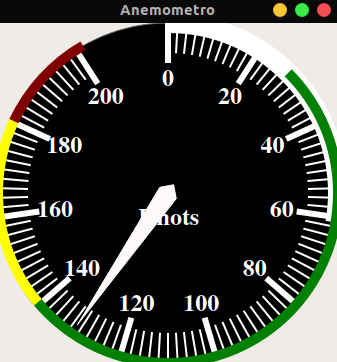
\includegraphics[width=0.4\textwidth]{anemometro.png}
	\caption*{Gauge para simular un anemómetro}
	\label{labelformat=empty}
\end{wrapfigure}

\paragraph{Software utilizado}
El software utiliza el paquete PyQt5. Este paquete viene a implementar las mismas características que Qt pero con la potencia del lenguaje Python. Mediante el dibujado de formas geométricas básicas es posible construir los instrumentos básicos de vuelo.\\

Los instrumentos virtuales representan la información recogida por los sensores y procesada por Arduino/Raspberry, que se asume como el controlador principal del UAV.

\paragraph{Mejoras del proyecto}

De momento los instrumentos sólo pueden ser llamados uno por uno, es decir, ejecutando sus scripts individualmente. La idea es incluir una ventana principal en la que el usuario pueda además de seleccionar de forma sencilla los elementos a mostrar, otras funcionalidades como mapas físicos, creadores de rutas de vuelo...

\begin{wrapfigure}{r}{0.5\linewidth}
	\centering
	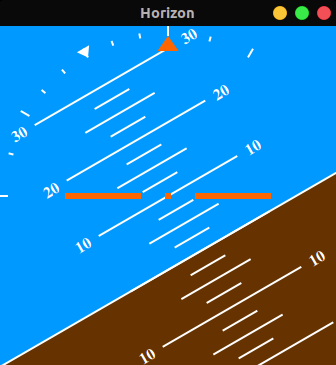
\includegraphics[width=0.40\textwidth]{horizonte.png}
	\caption*{Horizonte artificial en funcionamiento}
	\label{labelformat=empty}
\end{wrapfigure}

Una de las ideas fundamentales es la utilización de una antena capaz de servir como transceptor de datos entre la estación y la aeronave. Dado que mis conocimientos de telecomunicaciones son elementales comparados con un ingeniero de ese campo, esta parte del proyecto titulada "Long Range Com" está apartada por el momento.

\paragraph{Estado del proyecto}

El proyecto todavía no ha finalizado, pues a día de hoy soy el único contribuyente al mismo. Dado que es un proyecto largo y que no tiene relación directa con la Universidad, ha quedado en segundo plano dentro de mi lista de proyectos. Pero siempre que puedo trato de añadir alguna mejora al mismo.

\paragraph{Github}

Todos los códigos que componen los instrumentos pueden ser consultados en la cuenta de Github del autor. En particular el presente proyecto tiene su repositorio en: \href{https://github.com/jorgepiloto/falcon}{Proyecto Falcon}\\

Los pull-requests son bienvenidos, como en cualquier otro proyecto de open source.





